\documentclass[]{article}

\usepackage{graphicx}

\usepackage[margin=1in]{geometry}

\setlength\parindent{0pt}

\usepackage{physics}
% \usepackage{amsmath}

\usepackage{listings}

\usepackage{enumitem}
\renewcommand{\theenumi}{\alph{enumi}}

%opening

\title{MATH 5301 Elementary Analysis - Homework 1}

\author{Jonas Wagner}

\date{2021, September 01}



\begin{document}

\maketitle

\section{Problem 1}
\textbf{Problem:}
Prove the following tautologies by writing the true-false table.
Also translate each of these statements into human language.

\begin{enumerate}
	\item $A \lor \sim A$
	\item $(A \lor B) \Rightarrow A$
	\item $(A \land B) \Rightarrow A$
	\item $(A \Rightarrow B) \iff (\sim B \Rightarrow \sim A)$
	\item $\sim (A \lor B) \iff (\sim A \land \sim B)$
	\item $((A \Rightarrow B) \Rightarrow A) \Rightarrow A$
	\item $(A \Rightarrow (B \Rightarrow C)) \Rightarrow ((A \Rightarrow B) \Rightarrow (A \Rightarrow C))$
\end{enumerate}

\textbf{Solution:}\\
\begin{figure}[h]
	\centering
	\includegraphics*[width=0.7\textwidth]{fig/pblm1.png}
\end{figure}

\begin{enumerate}
	\item A or not A
	\item A or B implies A
	\item A and B implies A
	\item A implying B implies not B implying not A
	\item Neither A nor B occurs if and only if not A and not B
	\item A implying B implies A which implies A
	\item A implying B implies C implies that A implying B implies A implying C
\end{enumerate}

\newpage
\section{Problem 2}
\textbf{Problem:}
Prove the following identities for the set operations.
\begin{enumerate}
	\item $A \cap (B \cup C) = (A \cap B) \cup (A \cap C)$
	\item $(A \backslash B) \cup C = ((A \cup C) \backslash B) \cup (B \cap C)$
\end{enumerate}

\textbf{Solution:}
\begin{figure}[h]
	\centering
	\includegraphics*[width = \textwidth]{fig/pblm2a.png}
\end{figure}

\begin{figure}[h]
	\centering
	\includegraphics*[width = \textwidth]{fig/pblm2b.png}
\end{figure}

\newpage
\section{Problem 3}
\textbf{Problem:}
Write the following statements using quantifiers.
\begin{enumerate}
	\item Even elements of the sequence $\{a_n\}$ may be arbitrarly large.
	\item The sequence $\{a_n\}$ contains arbitary large even elements.
	\item The sequence $\{a_n\}$ contains infinitely many even elements.
\end{enumerate}

\textbf{Solution:}

\begin{enumerate}
	\item $\forall n \in \mathbf{N} : a_n \ \vdots \ 2 \Rightarrow \exists a \in \mathbf{N} : a_n \geq a$
	\item $\exists n \in \mathbf{N} : a_n \ \vdots \ 2 \Rightarrow \forall a \in \mathbf{N} : a_n > a$
	\item $\forall n \in \mathbf{N} : a_n \ \vdots \ 2 : \exists m \in \mathbf{N} : m > n : a_m \ \vdots \ 2$
\end{enumerate}

\newpage
\section{Problem 4}
\textbf{Problem:}
Show that:
\begin{enumerate}
	\item $\exists_x : (p(x) \lor q(x)) \iff (\exists_x : p(x)) \lor (\exists_x : q(x))$
	\item $(\forall_x p(x) \lor \forall_x q(x)) \Rightarrow \forall_x (p(x) \lor q(x))$
	\item Why is there no left arror implication on the previous line?
\end{enumerate}

\textbf{Solution:}\\
Part a)
\begin{figure}[h]
	\centering
	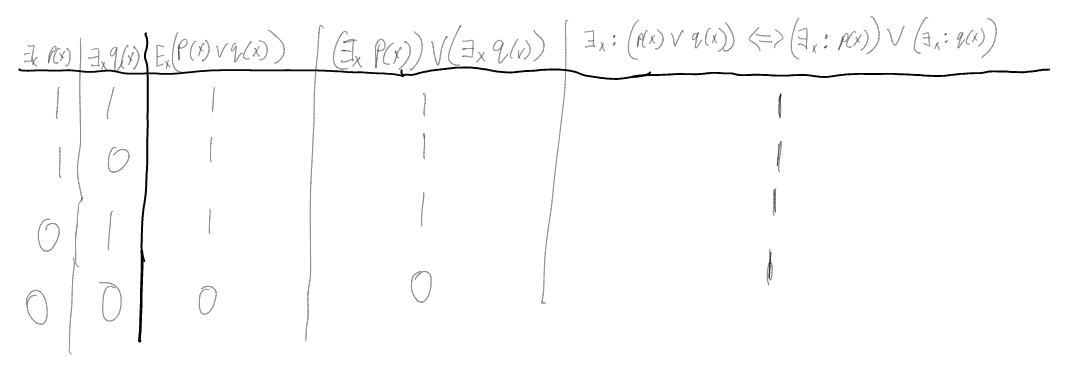
\includegraphics[width = \textwidth]{fig/pblm4a.png}
\end{figure}

Part b)
\begin{figure}[h]
	\centering
	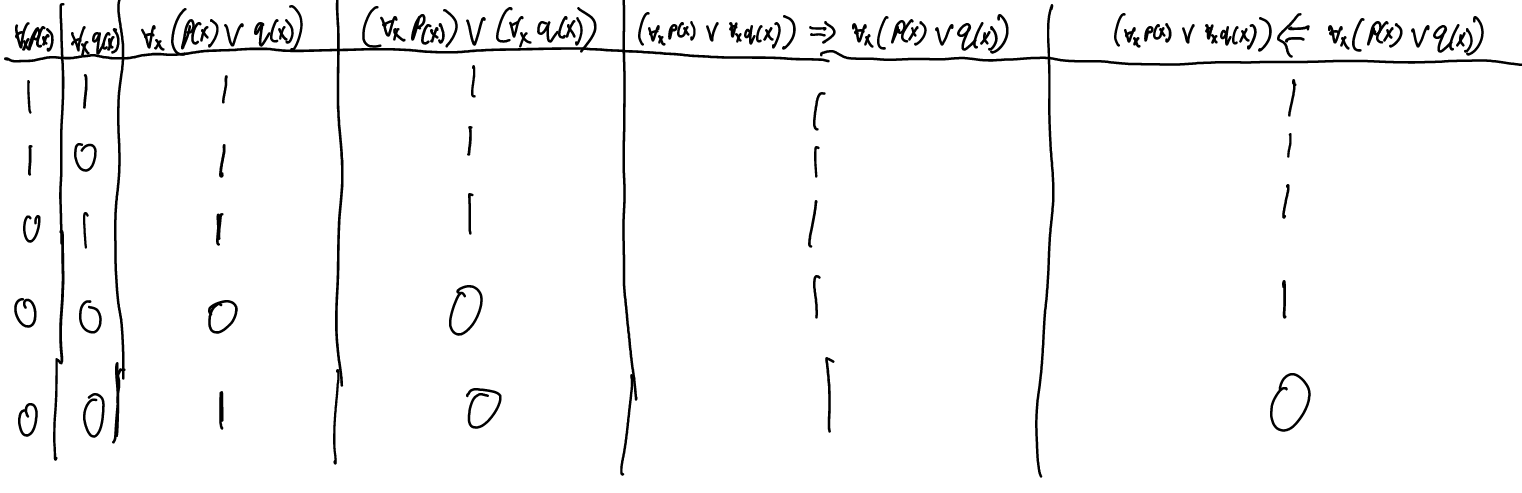
\includegraphics[width = \textwidth]{fig/pblm4b.png}
\end{figure}

Part c)\\
This is becouse there are cases when $p(x)$ and $q(x)$ themselves are not 
satisfied $\forall x$, but together at least one of them are true $\forall x$.


\newpage
\section{Problem 5}
\textbf{Problem:}
Show that one needs only one logic operation to construct all the 16 binary operations on statements A and B.\\
Define $A \star B$ via the following table:
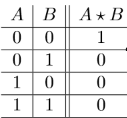
\includegraphics[width=0.3\textwidth]{fig/pblm5_star_TF_table.png}

Show that one can construct $\sim A, A \lor B, $and$ A \land B$ using only $\star$.
Then show that any other binary operation can be obtained from $\{\sim, \lor, \land\}$.\\

\textbf{Solution:}
\begin{figure}[h]
	\centering
	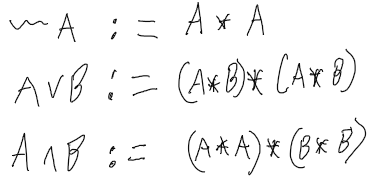
\includegraphics[width=0.7\textwidth]{fig/pblm5_star2op_soln.png}
	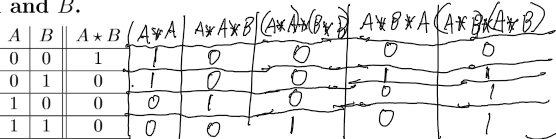
\includegraphics[width=0.9\textwidth]{fig/pblm5_star2op_table.png}	
\end{figure}

\newpage
(using the notation learned in digital circuits)\\
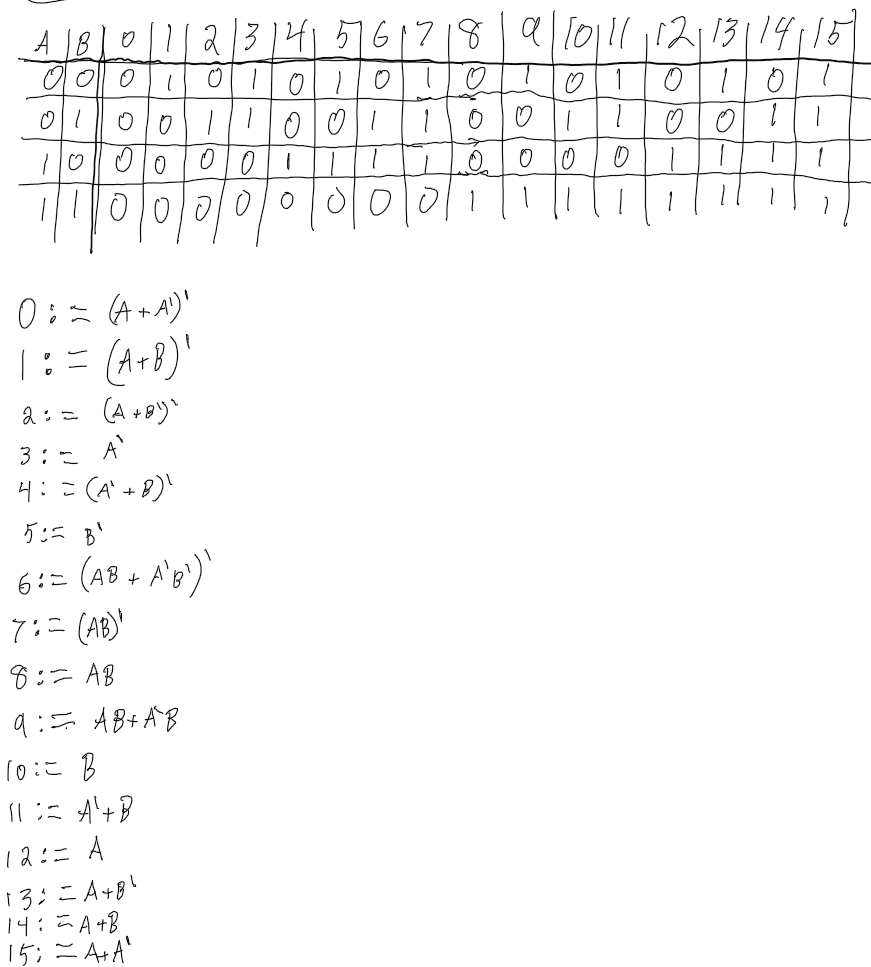
\includegraphics[width=\textwidth]{fig/pblm5_op2all_soln.png}


\newpage
\section{Problem 6}
\textbf{Problem:}
How many subsets does the set $A = \{a,p,p,l,e\}$ have?

\textbf{Solution:}
On the surface this problem can be solved simply by considering the selection of
each letter to be a part of a subset as a binary diget of T/F for inclusion,
resulting in $2^n = 2^5 = 32$.
However, due to the repeaterd element, $p$, this is not as simple but a similar
combinatorics proccess can be used to account for this.\\

\textbf{General Solution:}\\
Let the following be defined:\\
$n :=$ number of elements within $A$\\
$m :=$ number of unique elements within $A$\\
${a_i} :=$ sequence of the unique elements within $A$ ordered from 
the most occuring to the least occuring\\
${n_i} :=$ sequence of the number of unique elements, $a_i$, within $A$.\\
${(a_i,n_i)} := $ set of ordered pairs of unique elements of a unique
element, $a_i$, within $A$ paired with the number of $a_i$ elements contained
within $A$, $n_i$.\\

The calculation can split into the sum of all the possible subsets of lengths, $l$,
from 0 to n.\\
For $l=0$ the only possible subset is $\emptyset$,
so $$N_0 = \mqty(n \\ 0) = 1.$$

Similarily, for $l=n$ the only possible subset of $A$ is $A$, 
so $$N_n = \mqty(n \\ n) = 1.$$

For $l=1$ there exists $m$ unique sets consisting of the elements in $\{a_i\}$.
Alternativly, this can be calculated as
$$N_1 = \mqty(n\\1) - \sum_{i=1}^m (n_i - 1)$$.

For $l=2$ (and all $l>1$) the computation becomes more complicated.\\
The collection of subsets with repeated elements for $l=2$ would be all possible 
combinations of the elements of $A$ with $l=2$ elements, $\qty(N_{l=2}^{(all)} = \mqty(n\\2))$.\\

The number of duplicated elements can be done by constructing the ordered pairs 
$\{(b_i,n_i-1)\}: b_i = a_i \forall i : n_i > 1$. $B$ can then be defined as the collection 
of $n_i - 1$ copies of $b_i$. \footnote{How do you do this with quantifiers?}\\

The number of elements in $B$, $n^{(l=2)}$ can then be used to determine the number of duplicated 
subsets included in $N_{l=2}^{(all)}$, $N_{l=2}^{(duplicates)} = n^{(l=2)} * N_{l=1}$. Therefore,
$$N_{l=2} = N_{l=2}^{(all)} - N_{l=2}^{(duplicates)} 
= \mqty(n\\2) - n^{(l=2)} * N_{l=1} 
= \mqty(n\\2) - n^{(l=2)} * \qty(\mqty(n\\1) - \sum_{i=1}^m (n_i - 1))$$

This proccess can be repeated for $l > 2$ until the newly constructed set (labeled $B$ for $l=2$) is empty,
in which case $N_{l} = \mqty(n\\l)$.\\

For the given finite case of $A = \{a,p,p,l,e\}$ the result is calculated as:
\begin{align*}
	N_0 &= 1\\
	N_1 &= 4\\
	N_2 &= 13\\
	N_3 &= 6\\
	N_4 &= 4\\
	N_5 &= 1\\
	\intertext{Therefore,}
	N &= 29
\end{align*}
% One solution is to define the ordered pairs 
% $\{(b_i,n_i-1)\}: b_i = a_i \forall i : n_i > 1$. 
% The new sequence, $\{b_i\}$ can then be used to add the nessicary 
% extra repeated element subsets. 
% Additionally, let the number of elements within sequence $\{b_i\}$ 
% be defined as $m_2$. 
% The collection of subsets with $l=2$ would be all possible combinations of
% $a_i$, $\qty(N_{l=2}^{(all)} = \mqty(n\\2))$, minus the number of repeated
% subsets constructed with ${b_i,a_j} \forall i \in \{1,2,\cdots,m_2\}, 
% j \in \{1,2,\cdots,m_2\}$, $\qty(N_{l=2}^{(duplicates)} = m_2 * m)$. Therefore,
% $$N_2 = \mqty(m\\2) - m_2.$$

% Next, this proccess can be repeated for $2 < l < n$, such that a new set of
% ordered pairs is defined, $\{c_i, n + (l-1)\} : c_i = a_i \forall n > (l-1)$,
% and then the number of subsets with $l$ elements is calculated as
% the sum of all possible combinations of the elements of $A$ of length $l$, 
% $\qty(N_{l}^{(all)} = \mqty(n\\2))$, minus the number of repeated subsets
% constructed with ${c_i,\cdots,b_j,a_k} \forall i \in \{1,2,\cdots,m_l\},
% \cdots, j \in \{1,2,\cdots,m_2\}, k \in \{1,2,\cdots,m\}$, 
% $\qty(N_l)^{(duplicates)} = m_l * \cdots * m_2 * m$. Therefore,
% $$N_l = \mqty(n\\l) - m_l * \cdots * m_2 * m.$$

% The total number of possible subsets can then be calculated as the sum
% $$N = \sum_{l=1}^{n} N_l = \sum_{l=1}^n \mqty(n\\l) - \prod_{1}^{l} m_l$$

% Note: I am not overly confident of how well this scales when it grows
% larger then I actually tested it at...



\end{document}
